\newChapter{Domain specific language}
\label{cha:a-dsl}

\section{Introduction}
\label{sec:dsl_intro}

A \gls{DSL} is a programming language whose goal is
to provide a way to solve specific domain problems. For example, Matlab is a
domain specific language created to simplify matrix calculus.

What we call ``domain'' is a set of problem related together in the same scope.
For Matlab, those domains could be a matrix multiplication or the resolution of an
equation system. Those two operations are related to numerical mathematics and
that is the ``domain'' of Matlab.

This chapter introduces and discuss the question : ``Why use a DSL ?'' by
explaining the advantages that a \gls{DSL} could bring for domain-oriented
problems. Then we present the difference between an internal and an external DSL
and the advantages and disadvantages for both of them. Finally, we introduce the
implementation of a \gls{DSL} using the Scala programming language and why Scala
is a great tool for the development of \gls{DSL}.

\section{Why use a DSL ?}
\label{sec:why-use-dsl}

\gls{DSL} exist since the beginning of computing, according to
\cite{VanDeursen2000}, COBOL, Lisp and Fortran have been
created for solving problems in a specific area like business processing, numeric
computations or symbolic processing. With time, language has become more and
more generalist but \gls{DSL} has always been created to simplify some domain
specific problems.

Using a DSL instead of a programming language brings advantages as well as
disadvantages.

\textbf{Advantages:}
\begin{itemize}
\item A high potential of usability and reliability according to
  \cite{Tolvanen2010}.
\item A great learning curve because a DSL is, in general, easier to learn than a
  general programming language \cite{Mernik2005}.
\item An expert of the DSL could modify the application even without knowing how
  to program.
\end{itemize}

\textbf{Disadvantages \cite{VanDeursen2000}:}
\begin{itemize}
\item The cost to develop a DSL : production, user training and
  maintenance.
\item A non-expert user may find hard to modify an existing program.
\item In general, DSL are less efficient than general programming language,
  because programming languages own some very good compiler with a lot of
  optimisations.
\item The need to learn a new language, even if it's a simple one.
\item A DSL don't have any tool support (other than a compiler of course) \cite{Mernik2005}.
\end{itemize}

\section{Internal and External Domain specific language}
\label{sec:internal_and_external_dsl}

It exists two types of \gls{DSL} : internal \gls{DSL}, also call \gls{DSEL} and
external DSL. Understanding the difference, advantages and disadvantages of each
of those is crucial in order to create an appropriate solution to the domain
specific problems.

The main difference between this two concept appears at the compilation time,
the figure \ref{fig:internal_dsl_compilation} shows the compilation of an
internal DSL. The input and the output of the compiler are in the same language.
Then, the figure \ref{fig:external_dsl_compilation} shows the compilation of an
external DSL. This time, we compile the code into another language, called the host language.

\begin{figure}[ht]
  \centering
  \fbox{
    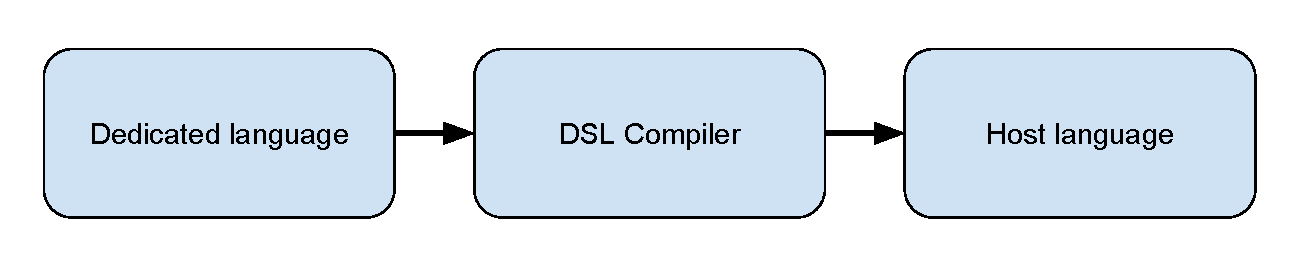
\includegraphics[width=0.8\textwidth]{img/internal_dsl_compilation}
  }
  \caption[Compilation process of an internal \gls{DSL}]{Compilation process of
    an internal Domain specific language. The input and output languages are the
    same. In general, we could see the input language as a library (with or
    without syntactic sugar) for more general programming language.}
  \label{fig:internal_dsl_compilation}
\end{figure}

\begin{figure}[ht]
  \centering
  \fbox{
    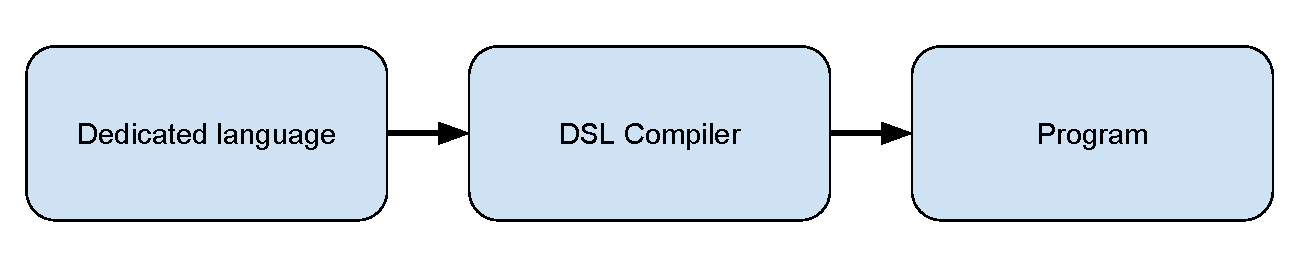
\includegraphics[width=0.8\textwidth]{img/external_dsl_compilation}
   }
  \caption[Compilation process of an external \gls{DSL}]{Compilation process of
    an external Domain specific language. The input and output languages aren't
    the same. This process is closer to a compiler for general language.}
  \label{fig:external_dsl_compilation}
\end{figure}

\subsection{Internal Domain Specific Language}
\label{sec:internal_dsl}

As shown in the figure \ref{fig:internal_dsl_compilation}, the dedicated language
and the output language are the same. Internal \gls{DSL} could be separate into
two categories : \gls{DEDSL} and \gls{SEDSL}.

Conceptually, a \gls{SEDSL} captures the semantic notions of the data's domain in
various data types and manipulate those data in a fixed way. Alternately, a
\gls{DEDSL} goes beyond the captures of semantic notions by capturing the
operations themselves. As an example for understanding those two concepts we look
at listing \ref{lst:deep_vs_shallow_source}. It's a small imaginary DSL used for
temperature manipulation between Kelvin and Celsius. We compute the sum
of three temperatures, and we want to print it in Celsius.

\begin{listing}[ht]
\centering
\begin{scalacode}
val t1 = Celsius(100)
val t2 = Celsius(50)
val t3 = Kelvin(30)
val t4 = t1 + t2 + t3
println(t4 in Celsius)
\end{scalacode}
\caption[Usage of the simple Temperature \gls{DSL}]{Example of the simple
Temperature \gls{DSL}. We simply want to compute the sum of three temperatures,
in Celsius and Kelvin, and finally want to print the result.}
\label{lst:deep_vs_shallow_source}
\end{listing}

Now we are going to compare the simple implementation of this \gls{DSL} for
both \gls{DEDSL} and \gls{SEDSL}. The implementation of the \gls{SEDSL} is
shown in listing \ref{lst:shallow_temp_scala} and for the \gls{DEDSL} in
listing \ref{lst:deep_temp_scala}.

\begin{listing}[ht]
\centering
\begin{scalacode}
sealed trait Temperature {
  def +(that : Temperature) = Add(this,that)
  def in(c : Celsius.type) = InCelsius(this)
}
case class Celsius(temp : Double) extends Temperature
case class Kelvin(temp : Double) extends Temperature
case class Add(t1 : Temperature, t2 : Temperature) extends Temperature
case class InCelsius(temperature: Temperature) extends Temperature
\end{scalacode}
\caption[Implementation of a \gls{SEDSL} for Temperature in
Scala]{Implementation of the simple Temperature \gls{SEDSL} with Scala, the
dedicated language is represented using an \gls{AST}, the values are never modified.}
\label{lst:shallow_temp_scala}
\end{listing}

\begin{listing}[ht]
\centering
\begin{scalacode}
import scala.language.implicitConversions

implicit def C2K(celsius: Celsius): Kelvin = Kelvin(celsius.temp + 273.15)
implicit def K2C(kelvin: Kelvin): Celsius = Celsius(kelvin.temp - 273.15)
implicit def T2K(temperature: Temperature): Kelvin = temperature match {
  case celsius: Celsius => C2K(celsius)
  case kelvin: Kelvin => kelvin
}
implicit def T2C(temperature: Temperature): Celsius = temperature match {
  case kelvin: Kelvin => K2C(kelvin)
  case celsius: Celsius => celsius
}

sealed abstract class Temperature(val tempInCelsius: Double) {
  def in(c: Celsius.type) = T2C(this)
  def in(k: Kelvin.type) = T2K(this)
  def +(that: Temperature): Temperature
}
case class Celsius(temp: Double) extends Temperature(temp) {
  override def +(that: Temperature): Temperature = add(that)

  private def add(that: Temperature): Celsius = {
    Celsius(T2C(that).temp + temp)
  }
}
case class Kelvin(temp: Double) extends Temperature(temp - 273.15) {
  override def +(that: Temperature): Temperature = add(that)

  private def add(that: Temperature): Kelvin = {
    Kelvin(T2K(that).temp + temp)
  }
}
\end{scalacode}
\caption[Implementation of a \gls{DEDSL} for Temperature in
Scala]{Implementation of the simple Temperature \gls{DEDSL} with Scala, the
dedicated language is represented directly by the host language primitives and
the data are directly manipulated.}
\label{lst:deep_temp_scala}
\end{listing}

In the case of a \gls{DEDSL}, we are directly using the primitives of the host
language. In this case, we use classes to represent a temperature. When we want
to combine the temperatures together, we create a new object and we apply the
transformation to the existing values as illustrate in the figure \ref{fig:dsl_deep_result}.

\begin{figure}[ht]
  \centering
  \begin{scalacode}
t1: Celsius = Celsius(100.0)
t2: Celsius = Celsius(100.0)
t3: Kelvin = Kelvin(100.0)
t4: Add = Add(Add(Celsius(100.0),Celsius(100.0)),Kelvin(100.0))

InCelsius(Add(Add(Celsius(100.0),Celsius(100.0)),Kelvin(100.0)))
  \end{scalacode}
  \caption[Result of the \gls{SEDSL} for Temperature]{Result of the small
    Temperature program from listing \ref{lst:deep_temp_scala}. The result
    represents the way to think about a \gls{SEDSL}. We capture the semantic of
    the computation.}
  \label{fig:dsl_shallow_result}
\end{figure}

With the \gls{SEDSL}, we save the \gls{AST} of the computation and we never
touch the values. The figure \ref{fig:dsl_shallow_result} shows the output for
the \gls{DEDSL}. The object is evolving over time.

\begin{figure}[ht]
  \centering
  \begin{scalacode}
t1: Celsius = Celsius(100.0)
t2: Celsius = Celsius(100.0)
t3: Kelvin = Kelvin(100.0)
t4: Temperature = Celsius(26.850000000000023)

Celsius(26.850000000000023)
  \end{scalacode}
  \caption[Result of the \gls{DEDSL} for Temperature]{Result of the small
    Temperature program from listing \ref{lst:deep_temp_scala}. The result
    represents the way to think about a \gls{DEDSL}. We capture the operations and
  we manipulate the information.}
  \label{fig:dsl_deep_result}
\end{figure}

In general, internal \gls{DSL} are closely related to the host language and some
of them are very good in this work. Language that offer operator overloading,
parametric polymorphism and functional mechanisms give a good user experience
and developer satisfaction as well.

\subsection{External Domain Specific Language}
\label{sec:external_dsl}

By opposition with an internal \gls{DSL}, an external \gls{DSL} is not built on
top of a host language. This kind of \gls{DSL} is completely independent from
any general programming language or another \gls{DSL}.

Developing an external \gls{DSL} needs additional work :
\begin{itemize}
\item A parser in order to recover the information from the source code.
\item A code generator.
\item Anything we want from other programming languages.
\end{itemize}

An external \gls{DSL} is very close to a programming language, except that a
\gls{DSL} is clearly simpler than a general programming language like C or Java.

\subsection{External vs Internal}
\label{sec:external_vs_internal}

External and internal \gls{DSL} are very different from each other. 
Understanding differences, strength and weaknesses is crucial for
further \gls{DSL} development.

\subsubsection{External \gls{DSL}}
\label{subsubsec:external_dsl}

External \gls{DSL} comes with the advantage that the \gls{DSL} designers may
define any possible syntax without any limitation\cite{strembeckmarkzdunuwe2009}. It could be textual,
graphical or even audiovisual (vocal command). Thus, because an external
\gls{DSL} is not bound to a specific host language or platform, the \gls{DSL}
could be used in any way and might be exported to additional target language or
platform through transformation \cite{strembeckmarkzdunuwe2009}. Finally, it's
almost impossible to accidentally use a feature that is not part of the \gls{DSL}
\cite{strembeckmarkzdunuwe2009}.

On the other hand, an external \gls{DSL} do not own any tool or support. There
is no compiler, no parser, no error checking, and so on. Everything as to be done
with the language creation.

\subsubsection{Internal \gls{DSL}}
\label{subsubsec:internal_dsl}

An internal \gls{DSL} always comes with a host language, and implies that the
\gls{DSL} designer and user have access to the features of the host language
\cite{strembeckmarkzdunuwe2009}. Moreover, all the tools related to the host
language are accessible. That includes : compiler, parser, debugger,
interpreters, code analysis tools and so on \cite{strembeckmarkzdunuwe2009}.

Another advantage of the internal \gls{DSL} is the support they have from
programming language. Some programming languages have a very good support by
default for the development and usage of \gls{DSL}. For example, Scala and Ruby
give some syntactic sugar which gives a pleasant way of development to the
user and designer.

In contrast to an external \gls{DSL}, the user of the \gls{DSL} may use some
features by accident and, at the runtime, the occurring errors could be
difficult to understand and not managed by the \gls{DSL} designer.

\section{Implementation of a Domain specific language with Scala}
\label{sec:implementation_of_a_dsl}

The Scala programming language has some great advantages over the other standard
programming languages like Java or C. This section will cover the implementation
of external and internal \gls{DSL} with Scala as well as some examples of
implementation. Finally, we will introduce the \gls{LMS} approach for internal
and external \gls{DSL}.

In order to illustrate the implementation of an external and internal \gls{DSL}
with Scala, we will create simple language which represents a calculator. The
\gls{DSL} will be able to parse a simple computation on natural numbers like $1 +
2 * 4$ and will compute the result and display it.

\subsection{External Domain Specific Language}
\label{subsec:scala_external_dsl}

External \gls{DSL} could be written in any programming language, from C to Java
via Haskell. The reason we use Scala is to be consistent with the internal
\gls{DSL} development. One of the goals of this thesis is to explore the
\gls{LMS} approach (available in section \ref{subsec:lms_approach}) for
\gls{DSL} development and this is a Scala oriented approach.

Implementing an external \gls{DSL} is quite the same as implementing a general
programming language. The difference is that it's simpler because the \gls{DSL}
is smaller than a programming language. In order to develop an external
\gls{DSL} we need the following components :

\begin{itemize}
\item Parser.
\item \gls{AST} representation.
\item Code generator or Interpreter.
\end{itemize}


The parsing part could be achieved with different libraries or framework. We can
also create or own tokenizer and parser from scratch. The advantage of that
technic is that we can optimise the parser and specialise it for the exact
syntax of our \gls{DSL}.

A big part of the parsing library in Scala is built using the parser combinator
method\cite{Odersky:2016:PSU:2988396}s. Basically, a parser combinator is a
\gls{HOF} that accepts some parsers in input and returns a parser. The parser is
a function that accepts a string in input and returns a structure in output. The
combination of several of those \gls{HOF} create parser which is more and more
complex.

Parser combinator in Scala is very similar to the \gls{EBNF} syntax. Listing
\ref{lst:Simple-calculator-parser} shows the parser for our little calculator \gls{DSL}.

\begin{listing}[ht]
\centering
\begin{scalacode}
class SimpleCalculatorParser extends RegexParsers with PackratParsers {
  override protected val whiteSpace: Regex = "[ \t\r\f\n]+".r

  override def skipWhitespace: Boolean = true

  lazy val simpleCalculatorProgram: PackratParser[Expr] = expr

  lazy val expr: PackratParser[Expr] = term

  lazy val term: PackratParser[Expr] = {
    term ~ "+" ~ product ^^ { case (l ~ _ ~ r) => Add(l, r) } |
      term ~ "-" ~ product ^^ { case (l ~ _ ~ r) => Sub(l, r) } |
      product
  }

  lazy val product: PackratParser[Expr] = {
    product ~ "*" ~ operand ^^ { case (l ~ _ ~ r) => Mul(l, r) } |
      product ~ "/" ~ operand ^^ { case (l ~ _ ~ r) => Div(l, r) } |
      operand
  }

  lazy val operand: PackratParser[Expr] = number | "(" ~> expr <~ ")"
  lazy val number: PackratParser[Expr] = "[0-9]+".r ^^ { str => Number(str.toInt) }
}
\end{scalacode}
\caption[Implementation of the simple calculator parser]{Implementation of the
simple calculator parser. The different parsers are combined, and they produce
the \gls{AST} for each expression separately before generating the whole structure.}
\label{lst:Simple-calculator-parser}
\end{listing}

The structures returned by a parser can be represented by a set of Scala classes
and traits. Case classes and the sealed modifier are perfect for such a
representation. The listing \ref{lst:Simple-calculator-ast} shows the
implementation of our simple calculator \gls{AST}. For example, the computation
$2 + 1 - 2$ is represented by \verb|Sub(Add(2,1),2)|.

\begin{listing}[ht]
\centering
\begin{scalacode}
sealed trait Expr
case class Number(value: Int) extends Expr
case class Add(left: Expr, right: Expr) extends Expr
case class Mul(left: Expr, right: Expr) extends Expr
case class Sub(left: Expr, right: Expr) extends Expr
case class Div(left: Expr, right: Expr) extends Expr
\end{scalacode}
\caption[\gls{AST} representation of the simple calculator \gls{DSL}]{\gls{AST}
representation of the simple calculator \gls{DSL}. Scala case classes and sealed
traits are very useful for this kind of representation.}
\label{lst:Simple-calculator-ast}
\end{listing}

Now we need to compute the result of the expression represented by the
\gls{AST}. We will just recursively walk into our AST, compute the
leaf and finally obtain the result of our expression. The listing
\ref{lst:Simple-calculator-interpreter} shows the interpreter for the simple
calculator \gls{DSL}. In a case of code generation, instead of returning the
evaluation of the \gls{AST}, we return to the set of operations that are necessary
to obtain the same result on a different platform or programming language.

\begin{listing}[ht]
\centering
\begin{scalacode}
sealed trait Expr {
  def eval: Int = this match {
    case Number(value) => value
    case Add(left, right) => left.eval + right.eval
    case Mul(left, right) => left.eval * right.eval
    case Sub(left, right) => left.eval - right.eval
    case Div(left, right) => left.eval / right.eval
  }
}
\end{scalacode}
\caption[Interpreter of the simple calculator \gls{DSL}]{Interpreter of the
simple calculator \gls{DSL}, each expression is evaluated recursively. In a case
of code generation, we don't return a result of the expression, but the
successive operations to get this result on another platform.}
\label{lst:Simple-calculator-interpreter}
\end{listing}

\subsection{Internal Domain Specific Language}
\label{subsec:scala_internal_dsl}

Scala is a great language for developing internal \gls{DSL}. The language itself
offer some great features, and syntactic sugar in order to create a user-friendly
syntax. Those advantages are the following \cite{filipkrikava2013}:

\begin{itemize}
\item Curried function.
\item Implicit function, class and parameters.
\item Omitting parenthesis.
\item No end statement symbol ('';'').
\item Infix operator syntax for methods.
\item Operator overloading.
\item \gls{HOF}.
\item By-name parameters evaluation.
\item Traits.
\item Definition of new type.
\end{itemize}

The listing \ref{lst:Simple-calculator-internal-dsl} shows the implementation of
our simple calculator using an internal representation. The usage of the
internal \gls{DSL} is different from the external one, but the semantic is the
same.

\begin{listing}[ht]
\centering
\begin{scalacode}
object Main extends SimpleCalculator {
  val a : int = 2
  val b : int = 3
  println(a + b - 3)
}

trait SimpleCalculator extends App {
  type int = ScInt

  sealed trait ScType {
    def +(that: ScType): ScType = (this, that) match {
      case (ScInt(a), ScInt(b)) => ScInt(a + b)
    }

    def -(that: ScType): ScType = (this, that) match {
      case (ScInt(a), ScInt(b)) => ScInt(a + b)
    }

    def *(that: ScType): ScType = (this, that) match {
      case (ScInt(a), ScInt(b)) => ScInt(a + b)
    }

    def /(that: ScType): ScType = (this, that) match {
      case (ScInt(a), ScInt(b)) => ScInt(a + b)
    }

    override def toString: String = this match {
      case ScInt(value) => s"$value"
    }
  }
  case class ScInt(value: Int) extends ScType

  implicit def Int2ScInt(int: Int) : ScInt = ScInt(int)
}
\end{scalacode}
\caption[Implementation of the simple calculator \gls{DSL}]{Implementation of
the simple calculator \gls{DSL}. The DSL is directly used in the code and
the implementation is showing some advantages of using Scala.}
\label{lst:Simple-calculator-internal-dsl}
\end{listing}

The listing \ref{lst:Simple-calculator-internal-dsl} is also showing some
features of Scala in action. The implicit definition \scalainline{int2ScInt} is used to
convert standard Scala Int into our special kind of Int named ScInt. We create
new methods named ``+'', ``-'', and so on and we used them with the infix
notation : \scalainline{2 + 3} is the same as \scalainline{2.+(3)}. By the way,
we are also using methods from the standard Scala library, in this case
\scalainline{println}, with our \gls{DSL}.

Finally, we could define new types with Scala. Listing
\ref{lst:Simple-calculator-internal-dsl} is not showing a great example,
but we can define type for everything. For example, a set of integer may be seen
as a function $Int \rightarrow Boolean$ so, in Scala, we could define the set
type with :

\scalainline{type Set[A] = A => Boolean}

Declaring new types is usefull for the \gls{DSL} designer as well as for the user
because the written code becomes clearer.

\subsection{The LMS approach}
\label{subsec:lms_approach}

\gls{LMS} is a Scala library, based on Scala-virtualized \cite{Rompf2012}, which
provided a runtime code generation approach
\cite{Rompf:2010:LMS:1942788.1868314}. The library as been created for providing
a way to create high-level \gls{DSL} and use staging to optimize the code
generated by the compiler.

The basic idea of \gls{LMS} is to represent two types of computation :
\begin{itemize}
\item the computations done at the compile time, noted $A$
\item the computations done at the runtime, noted $Rep[A]$
\end{itemize}

where $A$ is the type of the computation.

In order to illustrate this concept, look at the listing \ref{lst:lms-example}.
The idea is quiet the same, we want to call three times the function
{\normalsize \verb|doSomething|}. Now, we are going to generate the
corresponding scala code for each of those loops.

\begin{figure}[ht]
  \centering
\begin{scalacode}
def doSomething(i : Int) : Rep[Unit] = {
  println(i)
}

// A
for(i <- 0 until 3 : Range) {
  doSomething(i)
}

// Rep[A]
for(i <- 0 until 3 : Rep[Range]) {
  doSomething(i)
}
\end{scalacode}
  \caption[Difference between \(A\) and \(Rep\lbrack A\rbrack\) in a code example]{$A$ represent
    the value computed at the compile time and $Rep[A]$ represent the value
    computed at the runtime.}
  \label{lst:lms-example}
\end{figure}

\textbf{Loop $A$:}

The code \scalainline{0 until 3 : Range} is fully known at the compile time. So
the compiler don't have to produce a loop and produces the following :
\begin{scalacode}
doSomething(0)
doSomething(1)
doSomething(2)
\end{scalacode}

\textbf{Loop $Rep[A]$:}

The code \scalainline{0 until 3 : Rep[Range]} is not completely known at
the compile time. So the compiler will produce a loop in accordance with the
semantic of the operation.
\begin{scalacode}
var x = 0
while(x < 3) {
  val i = x
  doSomething(i)
  x += 1
}
\end{scalacode}

\section{Summary}
\label{sec:dsl_summary}

In this chapter we saw what is a \gls{DSL}, his advantages, disadvantages and
different kinds of \gls{DSL}. External \gls{DSL} could be seen as a programming
language with lesser features and domain-specific oriented. Internal \gls{DSL}
own two branches : \gls{DEDSL} and \gls{SEDSL}, each of those is designed and
built differently but also in a host language. Finally, we studied and
illustrated the implementation of any kind of \gls{DSL} using the Scala
programming and explained why Scala is a great language to build \gls{DSL} by
showing various libraries to create \gls{DSL}.

%%% Local Variables:
%%% mode: latex
%%% TeX-master: "../thesis"
%%% End:
